

\subsubsection{KW47: 01.11.2021 bis 08.11.2021}
\begin{quote}
	\subsubsection*{Arbeit in der Schule}
		Die Scenen von meinem Partner habe ich in den Ordner, wo meine Scenen sind hineinkopiert um sie nacher zu verbinden.
	\begin{figure}
		\centering
		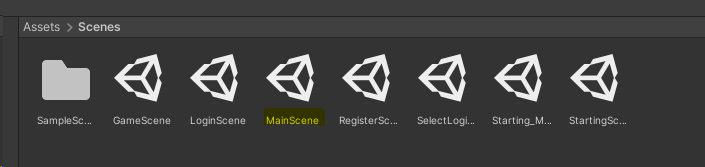
\includegraphics[width=0.7\linewidth]{img/SemihSoenmez_IMG/KW47_unity_scenes2}
		\caption{}
		\label{fig:kw47unityscenes2}
	\end{figure}
		Semih Can hat folgende Funktion programmiert: Wenn im Menü auf spielen gedrückt wird, wird der Main-Scene, wo unser Spiel ist gestartet. 
	
	\subsubsection*{Arbeit außerhalb der Schule}
	Kamera mit der Cinemachine-Funktion von Unity programmieren. Das Cinemachine Brain verwaltet alle virtuellen Kameras und entscheidet, welcher virtuelle Kamera die eigentliche Kamera folgen soll.
	
	\subsubsection*{Welche Schwierigkeiten hat es gegeben}

\end{quote}

